\section{Reducing The Branching Factor Further}
In this section we study two branching factor reduction methods: the first
is an offline perimeter pruning technique; the second is 
applied during individual node expansions.
Both retain the optimality of computed solutions (proofs omitted).

\noindent
\textbf{Perimeter Reduction:}
To speed up search we will prune all intermediate perimeter nodes: that is, nodes
which have no neighbours from any adjacent rectangle.
To preserve optimality, we will
connect the neighbours of each pruned node directly to each other.  The weight
of each new edge is set appropriately to the octile distance between the two
neighbours.  Figure \ref{fig-branching} (Left) shows an example.  

\begin{figure}[t]
	\begin{center}
	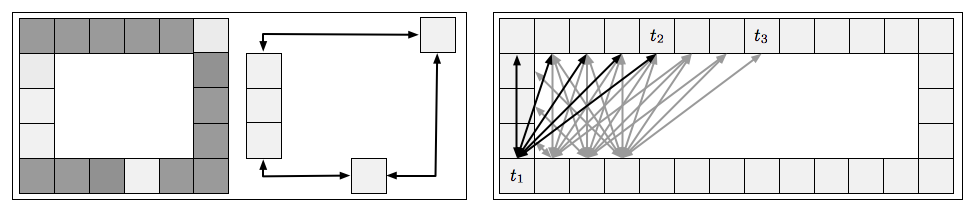
\includegraphics[width=0.97\columnwidth, trim = 10mm 10mm 10mm 0mm]
	{diagrams/branching_wide.png}
	\end{center}
	\vspace{-3pt}
	\caption{(Left) From each empty rectangle we prune all (dark grey) nodes which
	have no neighbours in any adjacent rectangle.
	Remaining nodes are then connected directly.
	(Right) Assume $t_{1}$ is the parent of $t_2$. When $t_2$
	is expanded, we do not generate neighbors from the opposite side.
	These can be reached from $t_1$ via a shorter or equal-length path.
}
\label{fig-branching}
\end{figure}

\noindent
\textbf{Online Node Pruning:}
When expanding a node during pathfinding search we observe that if the current
node, and its parent, both belong to the same rectangle, then it is not
necessary to consider any successors from the opposite side of the rectangle.
Figure \ref{fig-branching} (Right) shows an example of such a situation. 
When the current node has no parent, or the parent belongs to a different rectangle, 
we process all its successors.
